
\section{ビヘイビア駆動開発の実践}
CucumberとRSpecを用いてBDDでmy\_helpのテスト開発を進めていきました.
ビヘイビア駆動開発のコツとして「焦点を合わせる」ことが強調されています.
ここでは,焦点を合わせたmy\_helpの中での一つの振る舞いである
「todoの更新」を例として詳しく見ていきます.

\subsection{todoの更新マニュアル}
最初に,todoを更新するときの手順を示します.

\begin{enumerate}
\item my\_todo --editを入力して~/.my\_help/my\_todo.ymlを開く
\item editorでtodoを書き込む(今週やることならweeklyというitemを作ってそこに書き込む)
\item 保存して~/.my\_help/my\_todo.ymlを閉じる
\end{enumerate}
この振る舞いがきちんとできているのかをBDDでテストを書いていきます.

\subsection{Cucumber}
以下はtodoの更新を行うときのfeatureです.
まず,適当なディレクトリにfeaturesというディレクトリを作成します.
次に先ほど作成した,featuresディレクトリにmy\_todo.featureを作成します.
\begin{lstlisting}[style=customCsh,basicstyle={\scriptsize\ttfamily}]
# language: ja 

機能: todoの更新を行う
自分のするべきことを書き込むためにtodoを更新する

 シナリオ: コマンドを入力してtodoを更新していく
          前提 todoを編集したい
          もし "my_todo --edit"と入力する
          ならば editが開かれる
          かつ 自分のtodoを書き込む
\end{lstlisting}
機能とは,このシステムの機能のことを記述します.ここでは,todoを更新するシステムですので,「todoの更新を行う」です.
機能の下には,機能の補足説明を記述します.機能の補足説明では,ルールがないので自分がわかりやすいように,記述するのが常識です.
シナリオは,その名の通りtodoを更新する時のユーザの行動やシステム振る舞いを前提,もし,ならば,かつ,しかしに分類して記述します.

ここまでfeatureが記述できたら,次はcucumberコマンドを実行してみます.
コマンドは以下の通りです.
\begin{quote}\begin{verbatim}
nasu% cucumber features/my_todo.feature
\end{verbatim}\end{quote}
featuresディレクトリにあるmy\_todo.featureファイルをcucumberで実行するという意味です.

実行すると図\ref{fig:003}のようになります.

\begin{figure}[htbp]\begin{center}
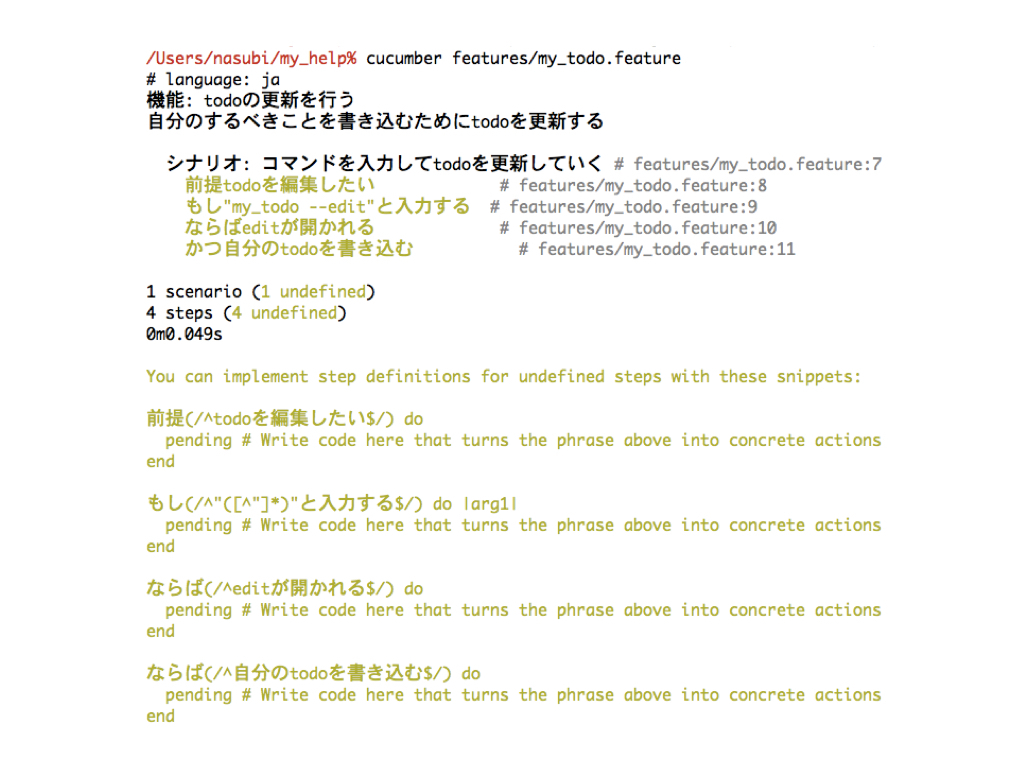
\includegraphics[width=12cm,bb= 0 0 937 753]{../figs/./my_help_nasu.003.jpeg}
\caption{step定義をする前のcucumberの実行結果.}
\label{fig:003}
\label{default}\end{center}\end{figure}
ここでは,1つのscenarioと4つのstepが失敗しています.
まだstep定義を記述していないので当たり前です.

一度cucumberを実行したのには理由があります.
featureを書いた時点でcucumberを実行すると,ステップ定義の元となるコマンドを,cucumberが自動的に作成してくれるからです.

以下がcucumberから出力されたステップ定義の元となる部分です.
\begin{lstlisting}[style=customCsh,basicstyle={\scriptsize\ttfamily}]
前提(/^todoを編集したい$/) do

end

もし(/^"([^"]*)"と入力する$/) do |command|

end

ならば(/^editが開かれる$/) do
  
end

ならば(/^自分のtodoを書き込む$/) do

end
\end{lstlisting}
これをコピーして,featuresディレクトリの中でstep\_definitionsディレクトリを作成し,その中にmy\_todo\_spec.rbを作成し,そこに貼付けます.

ここでもう一度cucumberを実行してみると図\ref{fig:004}のように変化が出てきます.

\begin{figure}[htbp]\begin{center}
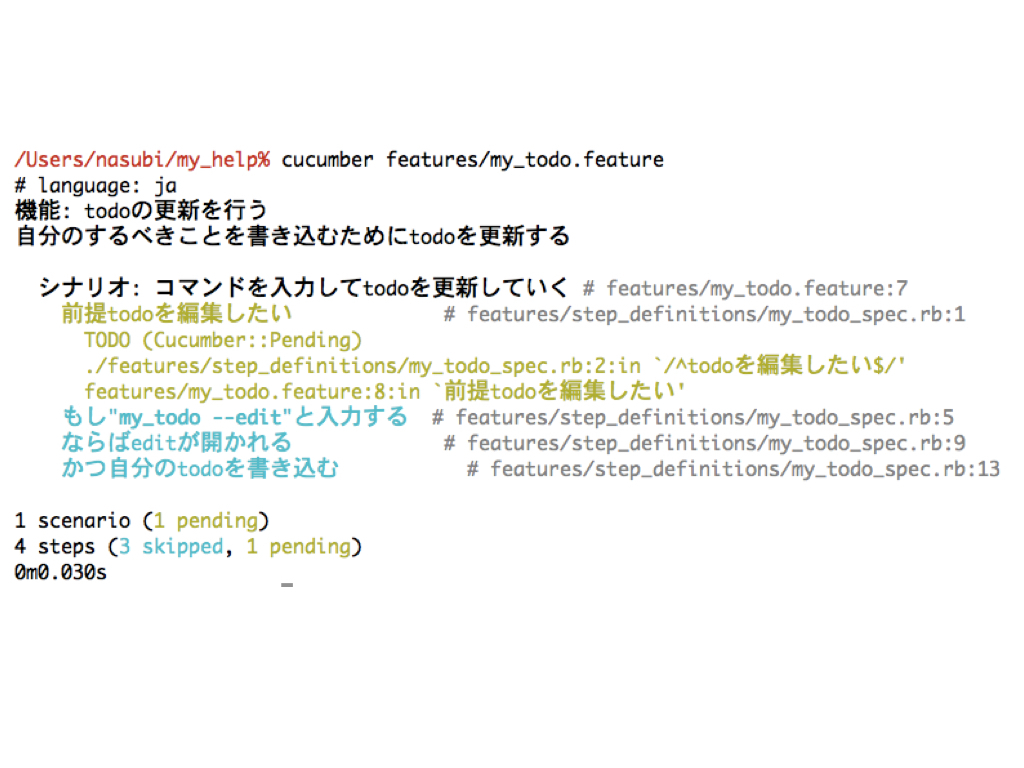
\includegraphics[width=12cm,bb= 0 0 937 753]{../figs/./my_help_nasu.004.jpeg}
\caption{defaultのstep定義を貼り付けた後のcucumberの実行結果.}
\label{fig:004}
\label{default}\end{center}\end{figure}
これは1つのシナリオがあり,1つがpendingであり,4つのstepの内1つがpendingで3つがskipしたことを表しています.
step\_definitionsのmy\_todo\_spec.rbのpending部分を書き換えて,step\_definitionsの記述を進めていきます.

まず,「前提」を見てみるとmy\_helpが何か振る舞いをすることはありません.
よって,このままにしておきます.
「もし」もユーザが入力するコマンドであり,my\_helpが何か振る舞いをすることはないのでこのままにしておきます.
次に,「ならば」を見てみるとmy\_helpがeditを開くという振る舞いをしています.
ステップ定義では,あれば良いと思うコードを記述するので私は下記のように記述しました.
\begin{lstlisting}[style=customCsh,basicstyle={\scriptsize\ttfamily}]
ならば(/^editが開かれる$/) do
  Mytodo::Edit.new.open
end
\end{lstlisting}
pendingの部分が書けたので,もう一度cucumber features/my\_todo.featureを実行します.
すると,図\ref{fig:005}のような結果が返ってきました.

\begin{figure}[htbp]\begin{center}
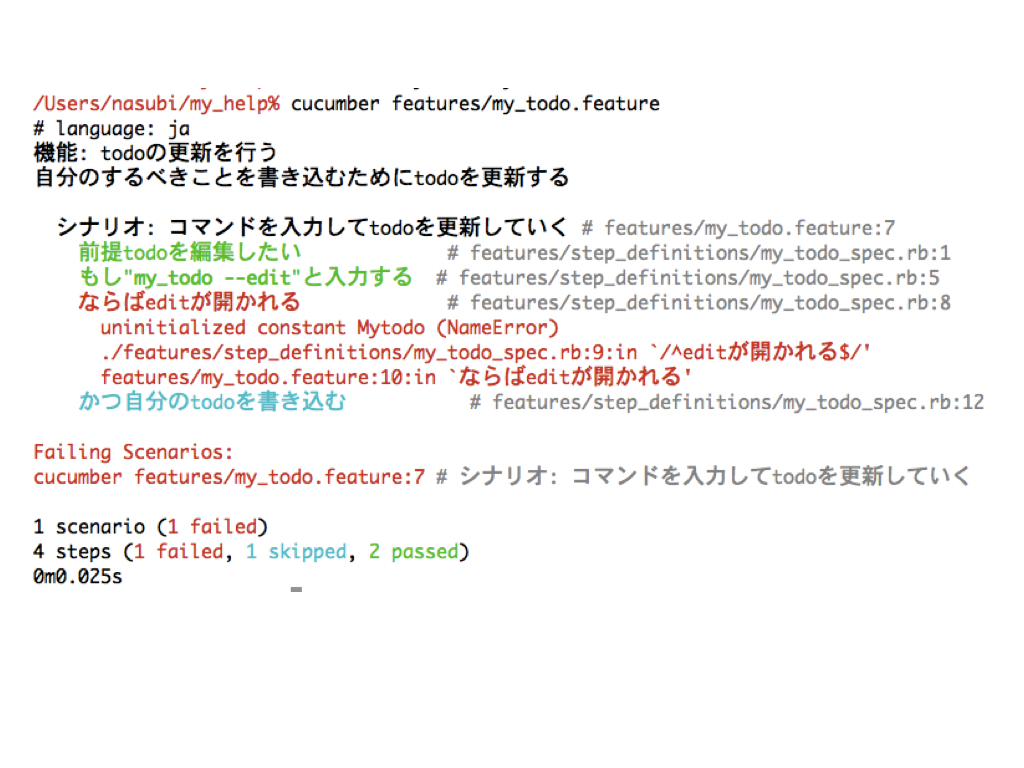
\includegraphics[width=12cm,bb= 0 0 937 753]{../figs/./my_help_nasu.005.jpeg}
\caption{pendingのstep定義を書き込んだ後のcucumberの実行結果.}
\label{fig:005}
\label{default}\end{center}\end{figure}
Cucumberは,エラーが出たステップのすぐ後ろにエラーを表示してくれます.
ここでCucumberでエラーが出たので,この「ならば editが開かれる」のシナリオに注目してRSpecに進むことにします.

\subsection{RSpec}
次にRSpecを使って実際にtodoを更新する振る舞いをするコード書いていきます.

そのための準備として,まずspecというディレクトリを作成し,my\_todoというサブディレクトリを追加します.
次に,このサブディレクトリにtodo\_spec.rbというファイルを追加します.
この機能はmy\_help --editと入力されれば,~/.my\_help/my\_todo.ymlが開かれるので,その振る舞いをするコードを書きます.
まずtodo\_spec.rbは下記の通りです.
\begin{lstlisting}[style=customRuby,basicstyle={\scriptsize\ttfamily}]
require 'spec_helper'


module Mytodo
  describe Todo do
    describe "#open" do
      it "open file my_todo.yml" 
    end
  end
end

\end{lstlisting}
describe()メソッドは,RSpecのAPIにアクセスしてRSpec::Core::ExampleGroupのサブクラスを返します.
ExampleGroupクラスはオブジェクトに期待される振る舞いのサンプルを示すグループです.
it()メソッドはサンプルを作成します.

完成したコードを下記の通りです.
\begin{lstlisting}[style=customRuby,basicstyle={\scriptsize\ttfamily}]
require 'spec_helper'


module Mytodo
  describe Todo do
    describe "#open" do
      it "open file my_todo.yml" do
          system("emacs ~/.my_help/my_todo.yml")
      end
    end
  end
end

\end{lstlisting}
specディレクトリのmy\_todoディレクトリをrspecで実行すると図\ref{fig:006}結果がでました.
\verb|--color|を付け加えるとわかりやすく色づけをしてくれて,見やすくなります.

\begin{figure}[htbp]\begin{center}
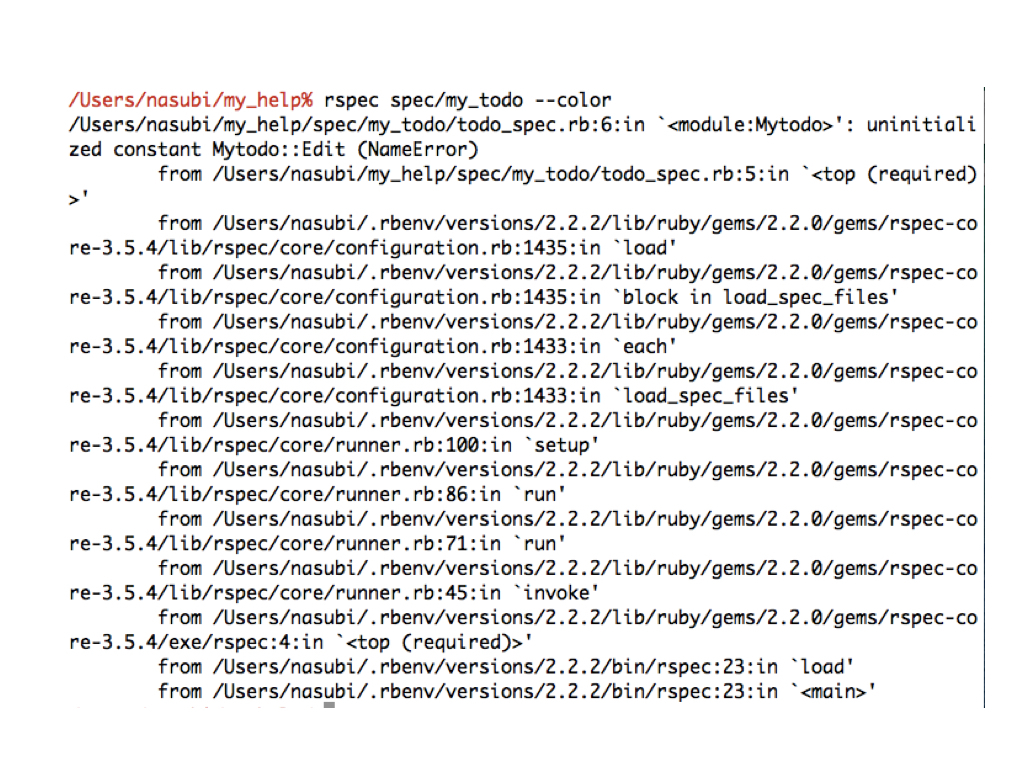
\includegraphics[width=12cm,bb= 0 0 937 753]{../figs/./my_help_nasu.006.jpeg}
\caption{pendingのstep定義を書き込んだ後のcucumberの実行結果.}
\label{fig:006}
\label{default}\end{center}\end{figure}
図\ref{fig:006}を見るとエラーが出てしまっているのがわかります.
\begin{quote}\begin{verbatim}
`<module:Mytodo>': uninitialized constant Mytodo::Edit (NameError)
\end{verbatim}\end{quote}
上記のエラーを解決するために,specディレクトリの一つ上の構造のディレクトリにlibディレクトリを作成します.
その中にmy\_todoというディレクトリを作成し,my\_todo.rbを作成します.

構造を表示すると以下のようになります.
\begin{quote}\begin{verbatim}
/Users/nasubi/my_help/lib/my_todo% ls
my_todo.rb
\end{verbatim}\end{quote}
my\_todo.rbに先ほどのエラーでMytodoというmoduleがないといわれているので,
ここで作成します.

/Users/nasubi/my\_help/lib/my\_todo/my\_todo.rbの中に以下のコードを記述します.
\begin{lstlisting}[style=customCsh,basicstyle={\scriptsize\ttfamily}]
module Mytodo
  class Edit
    def open

    end
  end
end
\end{lstlisting}
また,これをrequireしないといけないので,lib/todo.rbとして,以下を追加します.
\begin{quote}\begin{verbatim}
require 'my_todo/my_todo'
\end{verbatim}\end{quote}
これだけでは,rspecがlib/my\_todo/my\_todo.rbを読み込んでいないため,このスペックを実行するために,specディレクトリにspec\_helper.rbに以下を追加します.
\begin{lstlisting}[style=customCsh,basicstyle={\scriptsize\ttfamily}]
$LOAD_PATH.unshift File.expand_path('../../lib', __FILE__)
require 'todo'
\end{lstlisting}
これでもう一度rspecを実行してみると図\ref{fig:007}の結果が返ってきました.

\begin{figure}[htbp]\begin{center}
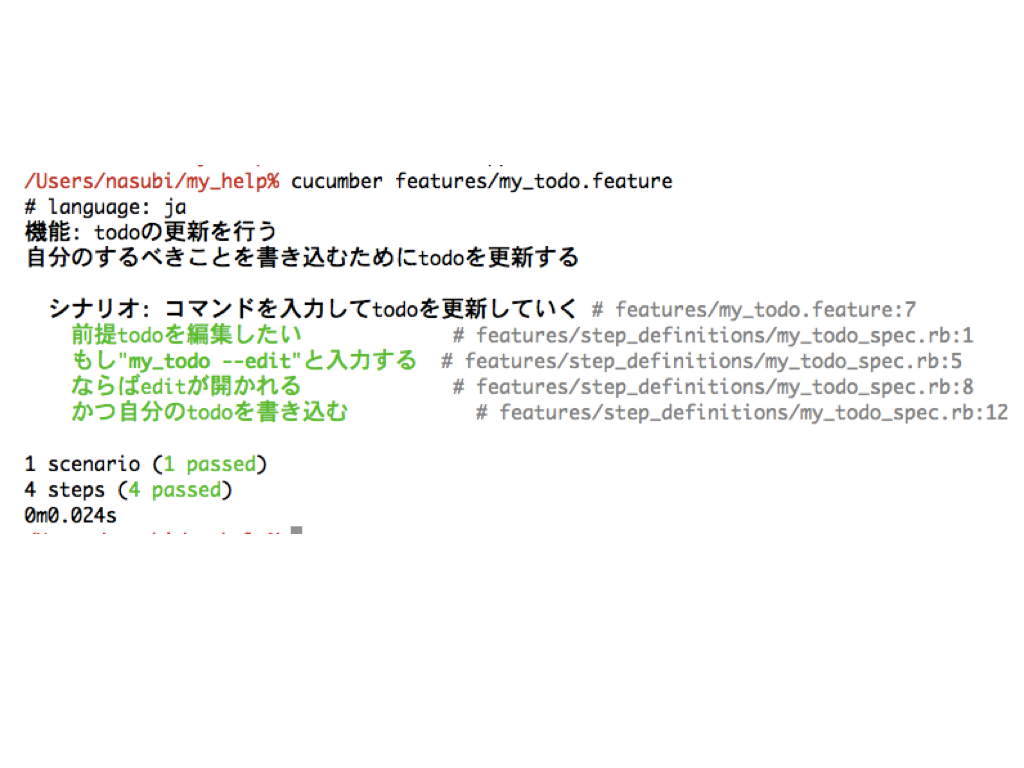
\includegraphics[width=12cm,bb= 0 0 937 753]{../figs/./my_help_nasu.007.jpeg}
\caption{redを修正してgreenになったrspecの実行結果}
\label{fig:007}
\label{default}\end{center}\end{figure}
図\ref{fig:007}を見ると,エラーが消えて成功しているのがわかります.
これで「ならば editが開かれる」のシナリオのRSpec部分が成功しました.
Red, Greenと進めたので次はRefactoringをするのですが,ここではあまり必要のないので省略します.
RSpecが終わったので,Cucumberに戻ります.

先ほどlibディレクトリでlib/my\_todo/my\_todo.rbを作成したので,cucumberでも読み込むために,以下を作成します.
\begin{quote}\begin{verbatim}
/Users/nasubi/my_help/features/support/env.rb
\end{verbatim}\end{quote}
env.rbの中は以下の通りです.
\begin{lstlisting}[style=customRuby,basicstyle={\scriptsize\ttfamily}]
$LOAD_PATH.unshift File.expand_path('../../../lib', __FILE__)
require 'todo'
\end{lstlisting}
これでcucumberもlib/の中身を読み取ってくれます.

もう一度cucumberを実行してみると,図\ref{fig:008}の結果が返ってきました.

\begin{figure}[htbp]\begin{center}
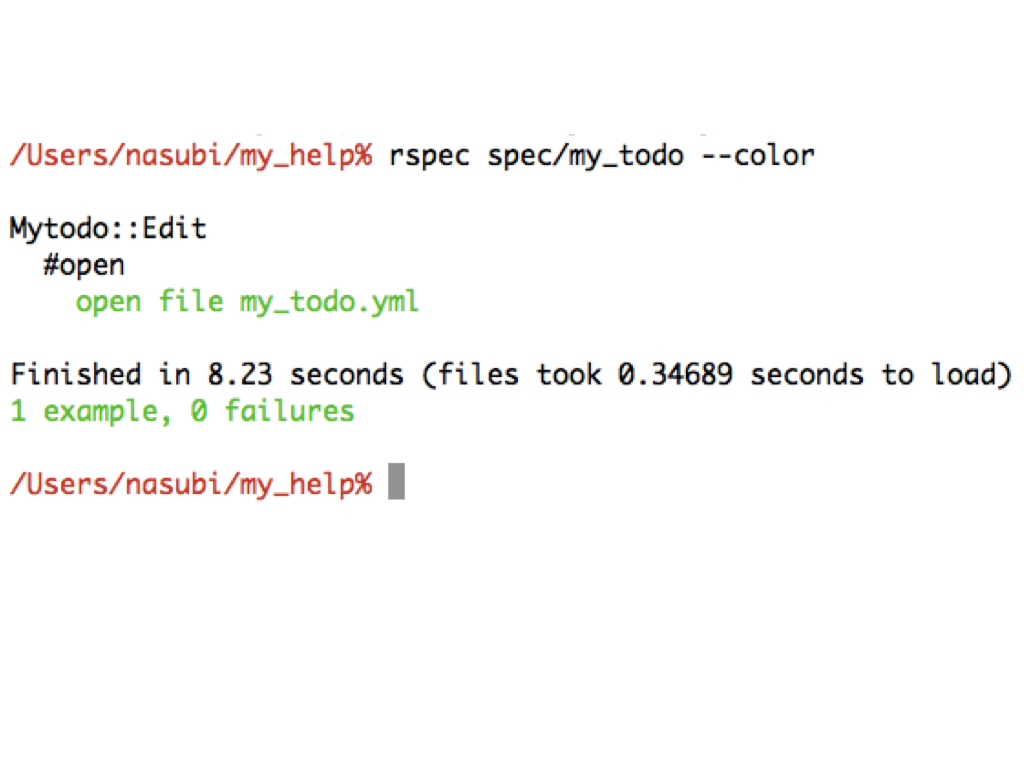
\includegraphics[width=12cm,bb= 0 0 937 753]{../figs/./my_help_nasu.008.jpeg}
\caption{libの中身を読み込むようにしたcucumberの実行結果.}
\label{fig:008}
\label{default}\end{center}\end{figure}
エラーが消えています.

これでBDDが成功しました.
残りの「自分のtodoを書き込む」もmy\_helpが何か振る舞いをするわけではないので,「コマンドを入力してtodoを更新する」シナリオ全てのテスト開発が終わりました.
このようにBDDでmy\_helpのテスト開発を行っていきました.

\subsection{.rspec options}
図\ref{fig:006}の時に述べたように,[rspec spec --color]で実行すると成功すればGreenで表示され,失敗すればRedで表示されます.
結果に色がついていると見やすく,どのような結果が出ているかが一目瞭然です.
しかし,毎回[--color]のコマンドを打ち込むのが面倒になってきます.
そこで,カレントディレクトリに.rspecを用意し,
\begin{quote}\begin{verbatim}
--format documentation
--color
\end{verbatim}\end{quote}
のようにすることで,rspecで実行するときにこのファイルを読み込み,[--color]を入力しなくても実行されます.

